\setcounter{chapter}{-1}
\chapter{Introduction}
This chapter will define the initial aspects of this project.
It will introduce the overall idea, which was inspired by the supervisor's project proposal.
It will then discuss what is required when designing mobile applications, and define a minimum viable product.
Since the project is concerned with a mobile application, the term \textit{mobility} will be explored.
Finally, the chapter introduces the process used for most of the development, making use of the \textit{Essence} process.

\section{Project idea}\label{sec:projectidea}
The idea for this project is to create a location-based competitive game using augmented reality (AR).
Two teams will compete against each other to score the most goals using a ball. 
Each player will be equipped with a smartphone-based virtual reality headset, and these will display the playing field from a top-down 2D view. 
To achieve this, each player's position needs to be tracked as well as where the ball is located on the field.
In the top-down view, each player needs to see the positions of the other players and the ball.
They also need to see their position on the playing field and where the goals are.
The players should be able to set a number of goals they need to score to win before beginning the game. 
\begin{figure}[H]
    \centering
    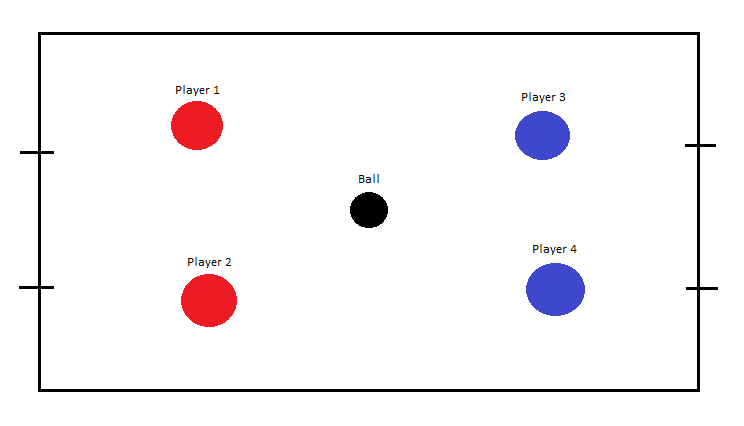
\includegraphics[width=0.6\linewidth]{Spil.PNG}
    \caption{An illustration of the playing field}
    \label{fig:game_illustration}
\end{figure}
\noindent
In \autoref{fig:game_illustration}, an illustration of the playing field for the game is shown.
There are goals at each end of the field, and the teams score goals by getting the ball between the goalposts.
An alternative version of the game is suggested where, instead of goals at each end of the field, there would be virtual goal zones seen in the game which the teams need to bring the ball into.
These zones could even change locations as the game progressed.

\subsection{Technical requirements for the project}
Various hardware will be required to realize the vision of the game.
First of all, each player must have a headset to hold their smartphone such that they can view a virtualized version of the playing field while playing.
In order for the data to be synchronized between the players, they will also need to be equipped with a positioning device, which can transmit their location to the other players.
This transfer of information will require a networking solution so that the virtualized playing field is synchronized between the players.

\subsection{Problems to consider}
The initial project idea proposes some problems that will need to be solved for the game to work.
We will need to consider which technologies to use for the development of the visual aspect of the game which should show a top-down view for each player. 
As we do not have experience creating VR-based games, it would be preferable if it is not necessary to have to build it from scratch.\\
Additionally, hardware that can track the positions of players and the ball is needed.
This must be accurate and update quickly such that the players do not run into each other, otherwise the game will not work.
Another problem to consider is how the ball should be displayed in a 2D view.
For the players to be able to find the ball on the field, it either has to be quite large to make it easier to find from the top-down view, or the game will need some metric to display how far the ball is from the ground.
The game will also need to track when the ball has crossed the goal line and then give feedback to the players.
Another problem to solve is how to keep the positional data synchronized across all the players' devices, as it will be difficult to play the game without accurate data.

\section{Designing for mobile devices}\label{sec:design-intro}
Designing for mobile devices requires that certain questions be clarified.
One of these questions is what type of device is being designed for, such as tablets, phones, or wearables.
Along with the type of device, certain things must be taken into account, such as the design language that is appropriate for the device, the way the device is interacted with,  how to facilitate touch interaction, as well as the different people expected to use the software being designed.
The main reasoning for having to think about design in this way is that users are not perfect.
They will not use the design the way the developers intended, they are different and use different devices, they are not designers themselves and they are unforgiving.
Ultimately, the users are not the problem, the design is.
In order to take this into account, we will establish requirements by looking at the context within which the game will be used and define a minimum viable product in \autoref{sec:mvp}.
We will also define prototypes for the design and finally evaluate it in the discussion section in \autoref{chap:conclusion}.

\section{Minimum viable product}\label{sec:mvp}
To be able to evaluate the game with users as fast as possible, we establish a minimal viable product with functional and non-functional requirements.
In \autoref{sec:design-intro} we explained how context is an important part of designing a mobile application.
Before establishing the requirements, the context will thus be analyzed.

\subsection{The context for the application}\label{subsec:context}
In terms of context, there is a distinction between \textit{Context} and \textit{context}.
\textit{Context} enables better understanding of a thing by adding information to it \cite{MobileDesign}.
In order to provide \textit{Context}, certain questions can be answered:
\begin{itemize}
    \item What problems are you designing a solution for?
    \item Who are the users, what is known about them and how will they interact with the design?
    \item What interaction is happening?
\end{itemize}
The problem the solution is designed for is the question of how to use Pozyx in order to create a virtual reality-based game.
The users will be from within a broad range, though they will requirement access to a positioning system, narrowing the range down.
The interaction happening is that the users will be able to define rules for the game, join it on a mobile phone and then play.
\\\\
Providing \textit{context} requires examining the mode, medium or environment in which the task is performed \cite{MobileDesign}.
It concerns itself with the requirements that need to be fulfilled in order for the \textit{Context} to work.
Questions related to this are:
\begin{itemize}
    \item Are there restrictions in environments?
    \item How are different devices present in different situations?
    \item Are there any prerequisites for interacting with the devices?
\end{itemize}
In terms of environments there is a restriction in that an internet connection will be necessary.
Outside of this connection, the game can be played both indoor and outdoor.
Since the game aims to incorporate a virtual reality-based aspect, the different devices present are mainly just phones for the players to view and play the game.
Finally, there is a prerequisite for interaction in that the size of the field needs to be known in order to facilitate an accurate representation of movement in a given space.


\subsection{Functional requirements}
These functional features are essential to make the game work and are the core features of the game.

\begin{itemize}
    \item Must be possible to start the game.
    \item The system must be mobile.
    \item Must be able to connect to the server from the clients.
    \item The users must be able to see their current positions.
    \item The users must be able to view the playing field, the goals, the players, the ball position, and the current score on their mobile device through VR goggles.
    \item A team must be able to win the game based on their score.
    \item The game must be dynamic, which includes:
          \begin{itemize}
              \item Support an arbitrary number of players.
              \item Size of the playing field can be set to a preferable size by the user.
              \item Set how many goals needed to score to win.
          \end{itemize}
\end{itemize}

\subsection{Non-functional requirements}
These requirements are more difficult to evaluate than the functional requirements and to test it a usability test must be conducted.
\begin{itemize}
    \item The design of the field must be pleasant for the user to look at through a VR headset.
    \item The users should receive enough updates so that the positions of the players represent their real position.
    \item The design of the system should support the context defined above in \autoref{subsec:context}.
\end{itemize}

\section{Mobility}\label{sec:mobility}
As a part of the study regulation it is emphasized that the system needs to be mobile.
The essence of the project idea as described in \autoref{sec:projectidea}, is that the players are mobile and easily can use their smartphone and virtual reality headset as the viewable device to view the game.
To achieve this form of mobility it requires us to handle wireless communication between users and by calculating the location of the players by the use of sensors.
\\\\
We also aim towards having the entire game as being mobile, which means that you would be able to set up the game at different locations.
This can however be more difficult, as some type of location-based service has to be used, as well as the need for connection between users to communicate.
Setting up the game at other locations also requires more knowledge about the game from the user, than the regular player otherwise would know, as the person has to set up the sensors at correct positions to measure the distance between the components.
\section{Our process}\label{sprint1:ourprocess}
%As described in \autoref{sec:essence}, a secondary focus of this project will be to attempt using the Essence process model as taught by the Software Innovation course.
This semester our process has been inspired by the \texttt{Essence} process taught in the Software Innovation course.
We have been working with a ScrumBut approach during previous semesters, but we decided that we wanted to try to improve our process by taking inspiration from a different process this semester.\\
However, we have chosen to keep sprints, stand-up meetings and retrospective meetings from Scrum as these can complement Essence.
To make the report fit this format, it has been split into 5 sprints that fit the length of the semester, with each sprint lasting three weeks, except for sprint 5 which will only last two weeks.
The main aspect of Essence we drew inspiration from was the team organization.

\subsection{Team organization in Essence}
\label{sec:team-organization}
Within the team organization, in Essence, roles are used to create heterogeneity in teams, to ensure diverse points of view and to ensure cohesion despite diversity.
The focus of these roles is to increase learning with personal interaction by sharing insights and experiences.
The roles also try to ensure that the team understands the problem domain, and that it sees the potential solutions in the technology domain.
\\\\
The roles are persistent as a rule of thumb, meaning that a member will have the same role for the duration of the project.
The roles in Essence are compatible with agile software development, making it possible to combine Essence with other processes like Scrum.
\\\\
There are four roles in Essence:
\begin{itemize}
    \item Child
    \item Responder
    \item Challenger
    \item Anchor
\end{itemize}
The role of \textit{Child} can ask any questions and make propositions that are in opposition to previous decisions.
The rest of the team is not allowed to criticize the \textit{Child}, but they are however allowed to ignore their suggestions.
The child is one of the main sources of ideas and other perspectives on the project.
\\\\
\textit{Responders} are the developers in the team, and are usually the majority within the team.
Responders work closely together with the \textit{Challenger}, so that the most important features are developed first.
\\\\
\textit{Challenger} is the customer or customer representative.
The challenger can be compared to the \textit{Product Owner} in Scrum.
This role formulates and explains the challenge, prioritizes features and accepts the solutions.
There can be more than one Challenger, but if there are they must agree on the product vision.
\\\\
The \textit{Anchor} is the one responsible for leading evaluations, but does not decide the consequences.
If necessary, the anchor can intervene and remove threats to the team's ability to develop ambitious responses.
A potential threat could be something that results in productivity issues.

\subsection{Roles in practice}
We have divided the roles described in \autoref{sec:team-organization} between the members of the group.
One member has the \textit{Challenger} role, meaning that they are accountable for prioritizing the tasks in the backlog.
The process of prioritizing tasks is further described in the following section.
Another member has the \textit{Anchor} role, and is responsible for changes to the process as well as in charge of leading the stand up meetings, retrospectives and evaluations of the process.
The rest of the group functions as \textit{Responders}, which is the role for the developers of the project.
The \textit{Child} role fluctuates between members of the group.
Everyone can add suggestions to improve an idea and give other perspectives on the project. \\
Due to our team size, the challenger and anchor will also work as developers during the duration of the project.

\subsection{Prioritizing tasks}
Our backlog is saved as a board on Jira, which can be seen on \autoref{fig:to-do-board}.
The leftmost column is the \textit{Suggested} column.
Everyone can make suggestions for tasks that they find useful for the project.
After each stand-up meeting, the challenger will present new suggestions that seem relevant to work on in the near future.
This presentation will include the definition of done, and all members of the group will then vote on how valuable it is for the project and how time-consuming it is.
The priority of a task is then calculated as $reward - time$, which is an arbitrary number to indicate how important it is.
\\\\
The challenger then chooses the most important features from the \textit{Discussed} column, often based on the highest priority, as \textit{Chosen for Development}.
Responders then have the opportunity to take tasks from this column and move it to the next column \textit{In progress} when they start working on it.
When the task has been completed, reviewed and merged into the develop branch, it is automatically moved to the column \textit{Done}.
\begin{figure}[H]
    \centering
    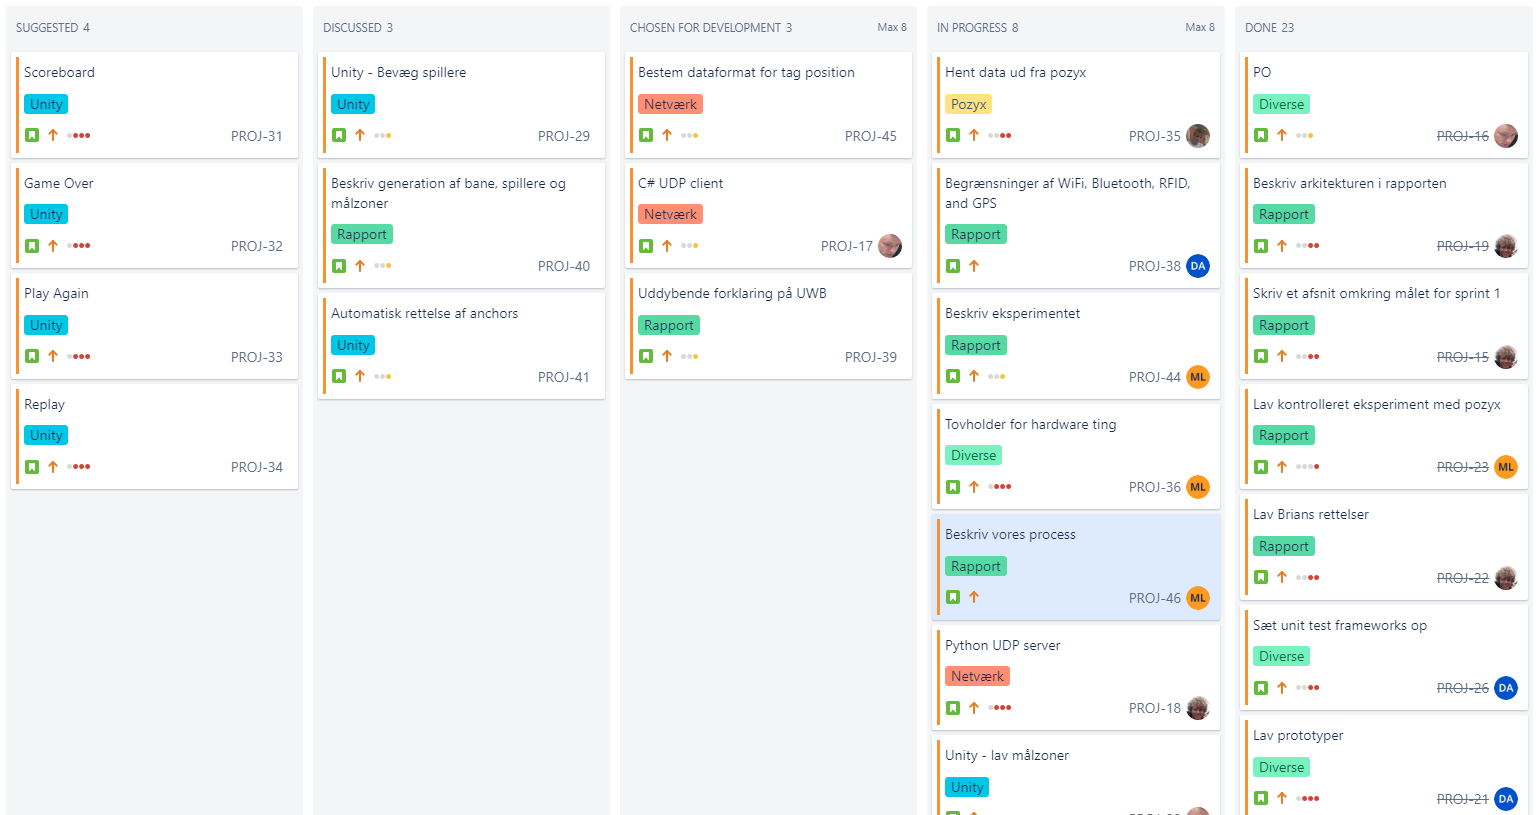
\includegraphics[width=\linewidth]{kanban.PNG}
    \caption{The board for tasks.}
    \label{fig:to-do-board}
\end{figure}

\subsection{Pair reviews}
Everything undergoes a formal review before it is added to the project in order to ensure quality.
This involves ensuring that the code is functional, implements the definition of done, is readable and makes sense, as well as accompanied by tests for parts of the system that might need it.
For report tasks, two reviewers are assigned to review and approve it before it can be merged.
For coding tasks, two people are likewise assigned to review it, but the review has to be done as a pair, meaning that they have to physically sit together and go through the code on a shared screen.
These pair reviews are a good way to share knowledge about the implementation through the group, as people have to understand it to be able to discuss it.
During previous semesters people have reviewed the code separately, which led to fewer comments as the code was not discussed between reviewers.

